\documentclass{article}
\usepackage[utf8]{inputenc}
\usepackage{listings} % Para código
\usepackage{graphicx} % Para gráficos
\usepackage{tikz} % Para dibujar gráficas

\lstset{ % Configuración para el código
    language=Python,
    basicstyle=\ttfamily\small,
    frame=single,
    numbers=left,
    numberstyle=\tiny,
    xleftmargin=2em,
    flexclrs=true,
    breaklines=true,
    postbreak=\mbox{\textcolor{red}{$\hookrightarrow$}\space},
}

\title{Búsqueda en Gráficas y Árbol Generador}
\author{Tu Nombre}
\date{\today}

\begin{document}
\maketitle

\section{Algoritmo de Búsqueda en Gráficas (BFS)}

El algoritmo presentado a continuación es una implementación de BFS (Búsqueda en Anchura):

\begin{lstlisting}
def search_in_graph(G, start_vertex):
    C = []
    colored = set()
    i = 0

    # Selecciona el vértice de inicio y colorea de negro
    r = start_vertex
    colored.add(r)
    C.append(r)
    print(f"Inicializando con vértice {r}")

    while C:
        r = C[0]
        neighbors = G[r]
        found_uncolored = False
        
        for y in neighbors:
            if y not in colored:
                i += 1
                colored.add(y)
                C.append(y)
                print(f"Vértice {y} coloreado y agregado a C")
                found_uncolored = True
                break
        
        if not found_uncolored:
            C.remove(r)
            print(f"Vértice {r} removido de C")

    print(f"Terminado. Todos los vértices han sido coloreados.")
\end{lstlisting}

\section{Gráfica G}

La gráfica \( G \) se describe con los siguientes vértices y aristas:

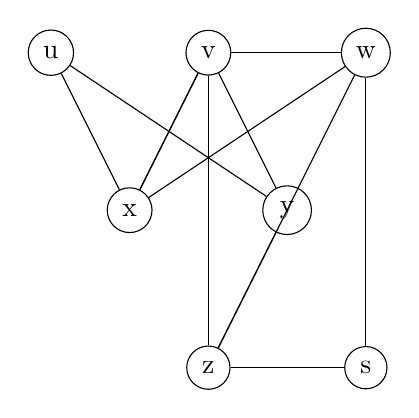
\begin{tikzpicture}
    \node[draw, circle] (u) at (0,2) {u};
    \node[draw, circle] (v) at (2,2) {v};
    \node[draw, circle] (w) at (4,2) {w};
    \node[draw, circle] (x) at (1,0) {x};
    \node[draw, circle] (y) at (3,0) {y};
    \node[draw, circle] (z) at (2,-2) {z};
    \node[draw, circle] (s) at (4,-2) {s};
    
    \draw (u) -- (x);
    \draw (u) -- (y);
    \draw (v) -- (x);
    \draw (v) -- (w);
    \draw (v) -- (y);
    \draw (v) -- (z);
    \draw (w) -- (x);
    \draw (w) -- (s);
    \draw (w) -- (z);
    \draw (x) -- (v);
    \draw (y) -- (z);
    \draw (z) -- (s);
\end{tikzpicture}

\section{Procedimiento}

Después de ejecutar el algoritmo de búsqueda en anchura con el vértice inicial \( u \), obtenemos el siguiente procedimiento:

\begin{enumerate}
    \item Inicializamos con el vértice \( u \).
    \item Exploramos vecinos de \( u \): \( x \) y \( y \). Coloreamos \( x \).
    \item Exploramos vecinos de \( x \): \( v \), \( w \). Coloreamos \( v \).
    \item Exploramos vecinos de \( v \): \( x \), \( w \), \( y \), \( z \). Coloreamos \( w \).
    \item Exploramos vecinos de \( w \): \( v \), \( x \), \( s \), \( z \). Coloreamos \( s \).
    \item Exploramos vecinos de \( s \): \( w \) y \( z \). Coloreamos \( z \).
    \item Exploramos vecinos de \( z \): \( y \). Coloreamos \( y \).
\end{enumerate}

El árbol generador resultante se puede describir mediante las aristas que fueron utilizadas para explorar nuevos vértices:

\[ u-x, x-v, v-w, w-s, s-z, z-y \]

\end{document}
